\section{splittable Task}

In the previous chapter we proposed an analytical model for execution time of a balanced parallel for loop in terems of the grain size, and based on this model, we offered an approach to find the range of grain size to achieve minimum exection time. The parameters of the propoesd model is identified through a benchmark and is exposed to the Blaze library to be used to predict the range of grain size for minimum excution time of a problem with a size that would be revealed at run-time. So the proposed solution is a combination of a compile-time and run-time solution to improve the performnace.
  
In this chapter we pick another direction and look into a run-time adaptive solution to control task granularity in order to achieve the minimum execution time. Why? unalanced work load.

In \cite{thoman2013adaptive}, the authors offer a combination of compile-time and run-time solution for adaptive control of task granulartity. They create multiple transformed versions of the code with differnet levels of task unrolling at compile time and then use a hueristic based on task demand (the number of unsuccesful steal attemps by other workers) and each worker's queue length, to select one of the versions each time a new task is spawned\cite{thoman2013adaptive}. Their solution relies completely on the compiler and the run-time, and eliminates the need for manual support.

In \cite{tzannes2014lazy}, the authors offer a run-time scheduling technique that adjusts the available parallelism based on the infered load at run-time, to avoid the unnecassary parallelism overhead. 

Splittable tasks are tasks that could be partitioned into smaller tasks, when sufficient parallelism is available\cite{prell2016embracing}. 

Utilizing splittable tasks is an approach to avoid creating large overhead of work stealing. 
Based on work stealing, in order to decrease the overhead of work stealing. 

\cite{aguilar2019line}


\subsection{Implementation}
For a for-loop with the range of $[a,b)$ one splittable task containg all the iterations from $a$ to $b-1$ would be created. Depending on the splitting strateg when a certain condition is met this task would be splitted into two parts, one containg iterations in the range of $[a,c)$ and the other part from $[c,b)$, where $c$ is the split point.   


In this talk I will briefly talk about Splittable Tasks and their implementation in HPX. Splittable task is a runtime adaptive method for managing task granulrity, to avoid the large overhead of creating and managing too many tasks caused by fine grain paralleism on one hand, and the starvation resulted from creating less tasks than available parallism on the other hand. Splittable tasks are tasks that could be partitioned into smaller tasks, when sufficient parallelism is available and are used as an adaptive runtime method to control task granulraity. I will discuss different strategies for splitting the tasks, which would result in creating different number of tasks, with different sizes, and will show the obtained results for a simple benchmark.   
 
\subsection{Splitting Strategies}
The splttable task could be splitted either based on total number of cores available, or number of idle cores at the time of split. 

\subsubsection{Splitting based on total number of cores}

\subsubsection{Splitting based on number of idle cores}

\subsection{Results}

\subsubsection{For-loop Benchmark}

\begin{figure}[H]
	\centering
	\subfloat[]
	{\centering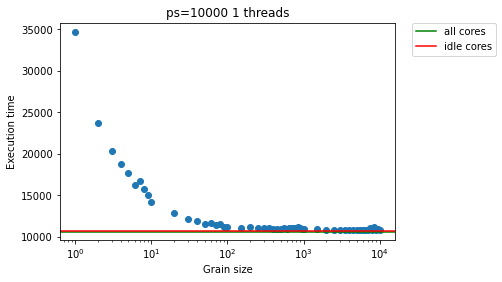
\includegraphics[scale=.35]{images/hpx_for_loop/splittable/all_idle_cores/marvin_10000_1.png}	
		\label{fig66:a}}
	\subfloat[]
	{\centering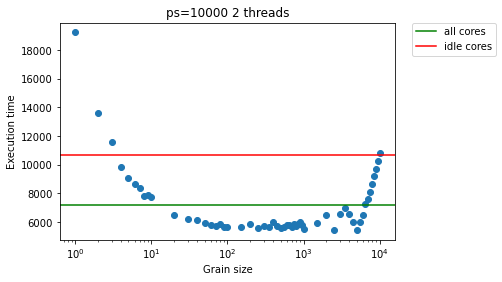
\includegraphics[scale=.35]{images/hpx_for_loop/splittable/all_idle_cores/marvin_10000_2.png}	
		\label{fig66:b}}\hfill
	\subfloat[]
	{\centering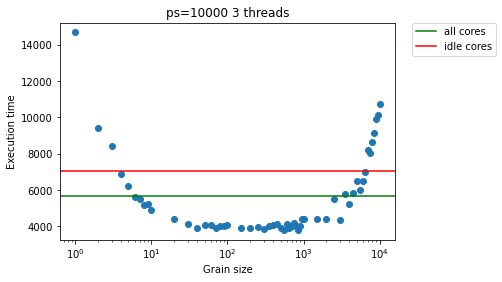
\includegraphics[scale=.35]{images/hpx_for_loop/splittable/all_idle_cores/marvin_10000_3.png}	
		\label{fig66:c}}
	\subfloat[]
	{\centering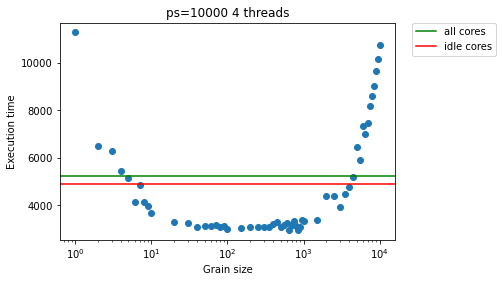
\includegraphics[scale=.35]{images/hpx_for_loop/splittable/all_idle_cores/marvin_10000_4.png}	
		\label{fig66:d}}\hfill
	\subfloat[]
	{\centering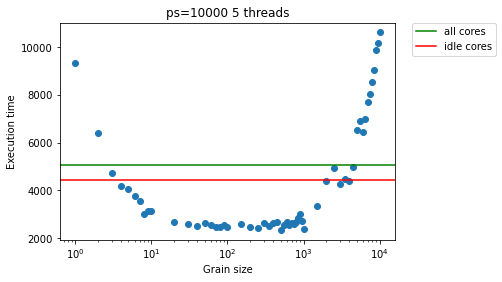
\includegraphics[scale=.35]{images/hpx_for_loop/splittable/all_idle_cores/marvin_10000_5.png}	
		\label{fig66:e}}
	\subfloat[]
	{\centering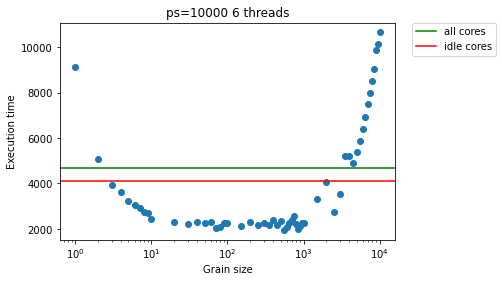
\includegraphics[scale=.35]{images/hpx_for_loop/splittable/all_idle_cores/marvin_10000_6.png}	
		\label{fig66:f}}\hfill
	\subfloat[]
	{\centering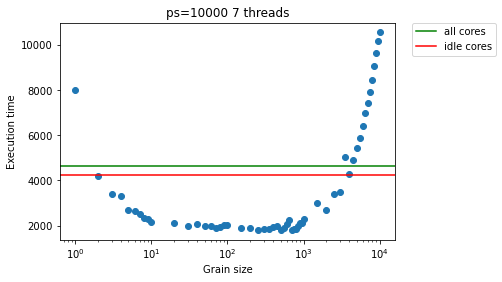
\includegraphics[scale=.35]{images/hpx_for_loop/splittable/all_idle_cores/marvin_10000_7.png}	
		\label{fig66:g}}
	\subfloat[]
	{\centering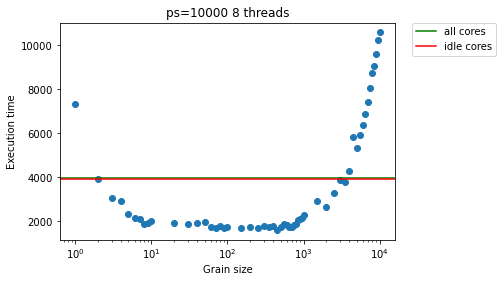
\includegraphics[scale=.35]{images/hpx_for_loop/splittable/all_idle_cores/marvin_10000_8.png}	
		\label{fig66:h}}\hfill
	\caption{The results of running the hpx for loop using splittable tasks with all-cores and idle-cores split types compared with different grain sizes, for $problem\_size=10000$, for (a) 1 core, (b) 2 cores, (c) 3 cores, (d) 4 cores, (e) 5 cores, (f) 6 cores, (g) 7 cores, (h) 8 cores. The unit for execution time is microseconds.}
	\label{fig66}	
\end{figure}

\subsubsection{Blazemark}